\documentclass[]{report}[12 pt]
\usepackage{geometry}
\usepackage{amsmath}
\usepackage{graphicx}
\usepackage{hyperref}
\geometry{margin= 1.5 cm}
\begin{document}
	\begin{titlepage}
	\begin{center}
		\vspace*{1cm}
		
		\Huge
		\textbf{Laboratory Report}
		
		\vspace{0.5cm}
		\LARGE
		X Ray Diffraction\\
		\vspace{0.5cm}
		\textbf{Guide: Prof. Sangita Bose}
		
		\vspace{1.5cm}
		
		\textbf{A R Bathri Narayanan}\\
		Roll no: P0211501\\
		UM DAE Centre for Excellence in Basic Sciences
		
		\vspace{3 cm}
		
		Report presented for the\\
		Advanced Physics Laboratory Course (PL 701)
		
		\vspace{0.8cm}
		
		
\includegraphics[width=0.4\textwidth]{cebs.jpg}
		
		\Large
		School of Physical Sciences\\
		UM-DAE Centre for Excellence in Basic Sciences\\
		Mumbai, MH, India\\
		\today
		
	\end{center}
\end{titlepage}

\section*{Objectives:}
\begin{enumerate}
	\item To study the IR characteristics of plasma with Langmuir probe.
	\item To study the dependence of obtained IR graph by varying pressure, voltage bias and resistance.
\end{enumerate}

\section*{Theory:}
The Nobel laureate Irving Langmuir made outstanding contributions in different fields of
Physics during the past century. He coined the term plasma in relation to the physics of
partially ionized gases and also invented the Langmuir probes to measure the electron plasma
density ne, the space potential Vsp and the electron temperature KBTe in cold low density
plasmas.\\
These Langmuir probes are one of the different electric probe diagnostics that are employed today. In
a broader sense, the electric probes measure the local
plasma parameters by using stationary or slow time
varying electric (and/or magnetic) fields to emit or
to collect charged particles from the plasma. These measuring techniques constitute an active field of research and are particularly well suited for low density cold plasmas, as low pressure electric discharges, iono-spheric and space plasmas.
The simplest collecting Langmuir probe is a metallic electrode (as those of Fig. 1) with a well defined geometry (planar, cylindrical or spherical). The probe is immersed into the plasma and polarized to the potential Vp by an external circuit. This bias to V = Vp-Vsp the probe with respect to the local space plasma potential Vsp. Then, the drained current Ip = I(Vp) for different probe potentials Vp is monitored and the plasma parameters are calculated from this voltage -
current (IV) characteristic curves.\\
However, behind this apparently simple scheme are hidden the intricate theoretical and
practical problems involved in the charge collection processes from a plasma.
\begin{center}
	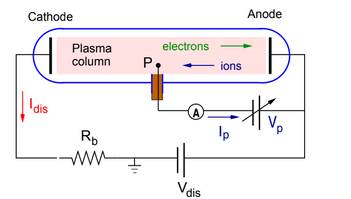
\includegraphics{lp1.png}\\
	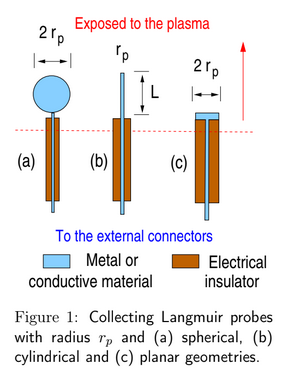
\includegraphics[width=6 cm]{lp2.png}
\end{center}
The plasma parameters are deduced from the current Ip, which, in accordance to the bias voltage V = Vp - Vsp is composed of ions, electrons or both. The attracted charges are collected by through the electric field between the bulk plasma and the metallic surface of the probe. This undetermined spatial potential profile extends in the plasma along distances in the order of few Debye lengths $\lambda$ D and is denominated plasma sheath. In
addition, this local electric field also may be altered according to the magnitude of the current Ip collected.
Therefore, the charge collection process depends on different characteristic lengths, as the probe size rp and the thickness (or spatial extension) of the plasma sheath attached to the collecting surface, which related with $\lambda$ D. In magnetized plasmas the electron re and ion ri Larmor radius also introduce additional lengths, as well as the mean free paths $\lambda$ for collisions between electrons and/or ions and neutral atoms
in collisional and weakly ionized plasmas.
\section*{Observations:}
We shall use a step voltage, so that we can study the IR characteristics in one shot.

\begin{center}
	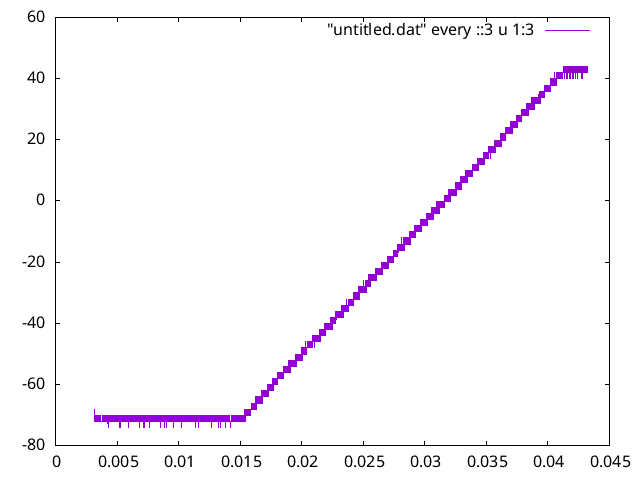
\includegraphics[width=10cm]{voltage}\\
	The step voltage take, the time is on x-axis and the voltage is on Y axis.
\end{center}
\subsection*{Variation of Pressure}
\begin{center}
	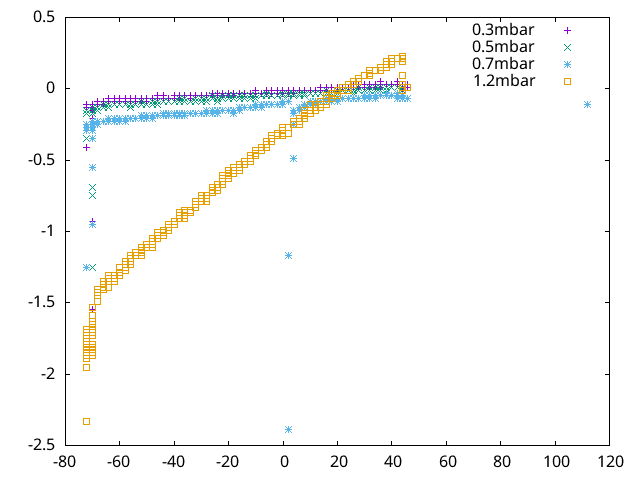
\includegraphics{variationpressure.png}\\
	V-I characteristics of the Plasma as we vary pressure.
\end{center}
We can see a non-linear variation of the graph as we increase the pressure. It first decreases and then increases. The reason might be due to the Paschen effect.
\[V = \frac{Bpd}{ln\bigg(\frac{Apd}{ln(1+\gamma^{-1})}\bigg)}\] 
At constant V, as we vary pressure, at first, it decreases and then it increases logarithmically.
\subsection*{Flipping the circuit}
\begin{center}
	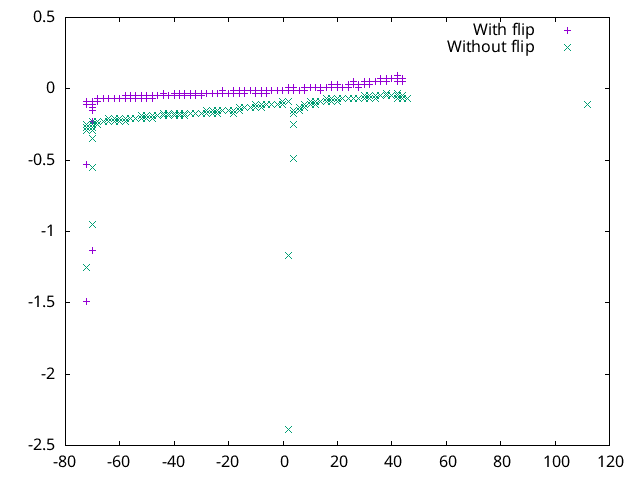
\includegraphics{flipping.png}\\
	V-I characteristics of the plasma as we flip the circuit.
\end{center}
We can see that the plasma when the ring is cathode is more stable with lesser fluctuations than it's counterpart. But except for a small deviation, the VI characteristics remain the same.

\subsection*{Variation of Bias Voltage}
\begin{center}
	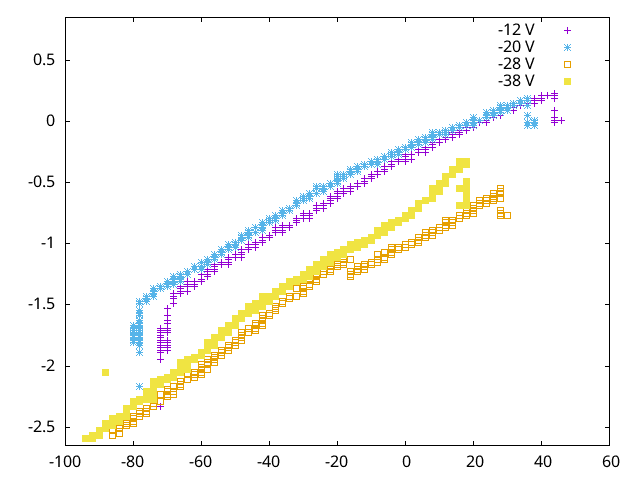
\includegraphics{variationbias.png}\\
	V-I characteristics of the plasma as we vary the bias voltage.
\end{center}
Bias voltage shows a general increasing trend as we vary it negatively, but it doesn't affect the slope of the graph.

\subsection*{Variation of Resistance}
\begin{center}
	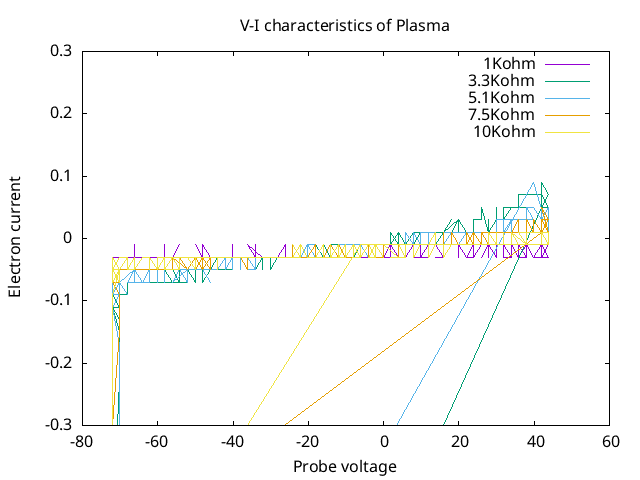
\includegraphics{variationresistance.png}\\
	V-I characteristics of the plasma as we vary resistance.
\end{center}
As we can see, as we increase the resistance, the temperature increases, so we see an increase in slope. At infinite resistance, we get to see the pattern more legibly.

\section*{Calculations:}
We can skip a few calculations, as slope only varies on Pressure and Resistance applied, we don't have to worry about the other quantities.
As the data is too noisy to perform actual calculation, we can eyeball calculations. The electron temperature of normal Argon is taken as 0.457 eV.\\
In case of pressure, the slope of the graph increases as we increase the pressure, so the electron temperature decreases, agreeing to the article called "Spectroscopic evaluation of vibrational temperature and electron density in reduced pressure radio frequency nitrogen plasma" By Hira Fatima et al.\\
As we increase the resistance, the slope increases, so the electron temperature decreases.

\section*{References}
Spectroscopic evaluation of vibrational temperature and electron density in reduced pressure radio frequency nitrogen plasma" By Hira Fatima et al.\\
An introduction to Langmuir probe diagnostics of plasmas, Luis Conde\\
\end{document}